% Options for packages loaded elsewhere
\PassOptionsToPackage{unicode}{hyperref}
\PassOptionsToPackage{hyphens}{url}
\PassOptionsToPackage{dvipsnames,svgnames,x11names}{xcolor}
%
\documentclass[
  letterpaper,
  DIV=11,
  numbers=noendperiod]{scrartcl}

\usepackage{amsmath,amssymb}
\usepackage{iftex}
\ifPDFTeX
  \usepackage[T1]{fontenc}
  \usepackage[utf8]{inputenc}
  \usepackage{textcomp} % provide euro and other symbols
\else % if luatex or xetex
  \usepackage{unicode-math}
  \defaultfontfeatures{Scale=MatchLowercase}
  \defaultfontfeatures[\rmfamily]{Ligatures=TeX,Scale=1}
\fi
\usepackage{lmodern}
\ifPDFTeX\else  
    % xetex/luatex font selection
\fi
% Use upquote if available, for straight quotes in verbatim environments
\IfFileExists{upquote.sty}{\usepackage{upquote}}{}
\IfFileExists{microtype.sty}{% use microtype if available
  \usepackage[]{microtype}
  \UseMicrotypeSet[protrusion]{basicmath} % disable protrusion for tt fonts
}{}
\makeatletter
\@ifundefined{KOMAClassName}{% if non-KOMA class
  \IfFileExists{parskip.sty}{%
    \usepackage{parskip}
  }{% else
    \setlength{\parindent}{0pt}
    \setlength{\parskip}{6pt plus 2pt minus 1pt}}
}{% if KOMA class
  \KOMAoptions{parskip=half}}
\makeatother
\usepackage{xcolor}
\setlength{\emergencystretch}{3em} % prevent overfull lines
\setcounter{secnumdepth}{-\maxdimen} % remove section numbering
% Make \paragraph and \subparagraph free-standing
\ifx\paragraph\undefined\else
  \let\oldparagraph\paragraph
  \renewcommand{\paragraph}[1]{\oldparagraph{#1}\mbox{}}
\fi
\ifx\subparagraph\undefined\else
  \let\oldsubparagraph\subparagraph
  \renewcommand{\subparagraph}[1]{\oldsubparagraph{#1}\mbox{}}
\fi

\usepackage{color}
\usepackage{fancyvrb}
\newcommand{\VerbBar}{|}
\newcommand{\VERB}{\Verb[commandchars=\\\{\}]}
\DefineVerbatimEnvironment{Highlighting}{Verbatim}{commandchars=\\\{\}}
% Add ',fontsize=\small' for more characters per line
\usepackage{framed}
\definecolor{shadecolor}{RGB}{241,243,245}
\newenvironment{Shaded}{\begin{snugshade}}{\end{snugshade}}
\newcommand{\AlertTok}[1]{\textcolor[rgb]{0.68,0.00,0.00}{#1}}
\newcommand{\AnnotationTok}[1]{\textcolor[rgb]{0.37,0.37,0.37}{#1}}
\newcommand{\AttributeTok}[1]{\textcolor[rgb]{0.40,0.45,0.13}{#1}}
\newcommand{\BaseNTok}[1]{\textcolor[rgb]{0.68,0.00,0.00}{#1}}
\newcommand{\BuiltInTok}[1]{\textcolor[rgb]{0.00,0.23,0.31}{#1}}
\newcommand{\CharTok}[1]{\textcolor[rgb]{0.13,0.47,0.30}{#1}}
\newcommand{\CommentTok}[1]{\textcolor[rgb]{0.37,0.37,0.37}{#1}}
\newcommand{\CommentVarTok}[1]{\textcolor[rgb]{0.37,0.37,0.37}{\textit{#1}}}
\newcommand{\ConstantTok}[1]{\textcolor[rgb]{0.56,0.35,0.01}{#1}}
\newcommand{\ControlFlowTok}[1]{\textcolor[rgb]{0.00,0.23,0.31}{#1}}
\newcommand{\DataTypeTok}[1]{\textcolor[rgb]{0.68,0.00,0.00}{#1}}
\newcommand{\DecValTok}[1]{\textcolor[rgb]{0.68,0.00,0.00}{#1}}
\newcommand{\DocumentationTok}[1]{\textcolor[rgb]{0.37,0.37,0.37}{\textit{#1}}}
\newcommand{\ErrorTok}[1]{\textcolor[rgb]{0.68,0.00,0.00}{#1}}
\newcommand{\ExtensionTok}[1]{\textcolor[rgb]{0.00,0.23,0.31}{#1}}
\newcommand{\FloatTok}[1]{\textcolor[rgb]{0.68,0.00,0.00}{#1}}
\newcommand{\FunctionTok}[1]{\textcolor[rgb]{0.28,0.35,0.67}{#1}}
\newcommand{\ImportTok}[1]{\textcolor[rgb]{0.00,0.46,0.62}{#1}}
\newcommand{\InformationTok}[1]{\textcolor[rgb]{0.37,0.37,0.37}{#1}}
\newcommand{\KeywordTok}[1]{\textcolor[rgb]{0.00,0.23,0.31}{#1}}
\newcommand{\NormalTok}[1]{\textcolor[rgb]{0.00,0.23,0.31}{#1}}
\newcommand{\OperatorTok}[1]{\textcolor[rgb]{0.37,0.37,0.37}{#1}}
\newcommand{\OtherTok}[1]{\textcolor[rgb]{0.00,0.23,0.31}{#1}}
\newcommand{\PreprocessorTok}[1]{\textcolor[rgb]{0.68,0.00,0.00}{#1}}
\newcommand{\RegionMarkerTok}[1]{\textcolor[rgb]{0.00,0.23,0.31}{#1}}
\newcommand{\SpecialCharTok}[1]{\textcolor[rgb]{0.37,0.37,0.37}{#1}}
\newcommand{\SpecialStringTok}[1]{\textcolor[rgb]{0.13,0.47,0.30}{#1}}
\newcommand{\StringTok}[1]{\textcolor[rgb]{0.13,0.47,0.30}{#1}}
\newcommand{\VariableTok}[1]{\textcolor[rgb]{0.07,0.07,0.07}{#1}}
\newcommand{\VerbatimStringTok}[1]{\textcolor[rgb]{0.13,0.47,0.30}{#1}}
\newcommand{\WarningTok}[1]{\textcolor[rgb]{0.37,0.37,0.37}{\textit{#1}}}

\providecommand{\tightlist}{%
  \setlength{\itemsep}{0pt}\setlength{\parskip}{0pt}}\usepackage{longtable,booktabs,array}
\usepackage{calc} % for calculating minipage widths
% Correct order of tables after \paragraph or \subparagraph
\usepackage{etoolbox}
\makeatletter
\patchcmd\longtable{\par}{\if@noskipsec\mbox{}\fi\par}{}{}
\makeatother
% Allow footnotes in longtable head/foot
\IfFileExists{footnotehyper.sty}{\usepackage{footnotehyper}}{\usepackage{footnote}}
\makesavenoteenv{longtable}
\usepackage{graphicx}
\makeatletter
\def\maxwidth{\ifdim\Gin@nat@width>\linewidth\linewidth\else\Gin@nat@width\fi}
\def\maxheight{\ifdim\Gin@nat@height>\textheight\textheight\else\Gin@nat@height\fi}
\makeatother
% Scale images if necessary, so that they will not overflow the page
% margins by default, and it is still possible to overwrite the defaults
% using explicit options in \includegraphics[width, height, ...]{}
\setkeys{Gin}{width=\maxwidth,height=\maxheight,keepaspectratio}
% Set default figure placement to htbp
\makeatletter
\def\fps@figure{htbp}
\makeatother

\KOMAoption{captions}{tableheading}
\makeatletter
\makeatother
\makeatletter
\makeatother
\makeatletter
\@ifpackageloaded{caption}{}{\usepackage{caption}}
\AtBeginDocument{%
\ifdefined\contentsname
  \renewcommand*\contentsname{Table of contents}
\else
  \newcommand\contentsname{Table of contents}
\fi
\ifdefined\listfigurename
  \renewcommand*\listfigurename{List of Figures}
\else
  \newcommand\listfigurename{List of Figures}
\fi
\ifdefined\listtablename
  \renewcommand*\listtablename{List of Tables}
\else
  \newcommand\listtablename{List of Tables}
\fi
\ifdefined\figurename
  \renewcommand*\figurename{Figure}
\else
  \newcommand\figurename{Figure}
\fi
\ifdefined\tablename
  \renewcommand*\tablename{Table}
\else
  \newcommand\tablename{Table}
\fi
}
\@ifpackageloaded{float}{}{\usepackage{float}}
\floatstyle{ruled}
\@ifundefined{c@chapter}{\newfloat{codelisting}{h}{lop}}{\newfloat{codelisting}{h}{lop}[chapter]}
\floatname{codelisting}{Listing}
\newcommand*\listoflistings{\listof{codelisting}{List of Listings}}
\makeatother
\makeatletter
\@ifpackageloaded{caption}{}{\usepackage{caption}}
\@ifpackageloaded{subcaption}{}{\usepackage{subcaption}}
\makeatother
\makeatletter
\@ifpackageloaded{tcolorbox}{}{\usepackage[skins,breakable]{tcolorbox}}
\makeatother
\makeatletter
\@ifundefined{shadecolor}{\definecolor{shadecolor}{rgb}{.97, .97, .97}}
\makeatother
\makeatletter
\makeatother
\makeatletter
\makeatother
\ifLuaTeX
  \usepackage{selnolig}  % disable illegal ligatures
\fi
\IfFileExists{bookmark.sty}{\usepackage{bookmark}}{\usepackage{hyperref}}
\IfFileExists{xurl.sty}{\usepackage{xurl}}{} % add URL line breaks if available
\urlstyle{same} % disable monospaced font for URLs
\hypersetup{
  pdftitle={Modelling Country Effect IMR differences},
  pdfauthor={Jon Minton},
  colorlinks=true,
  linkcolor={blue},
  filecolor={Maroon},
  citecolor={Blue},
  urlcolor={Blue},
  pdfcreator={LaTeX via pandoc}}

\title{Modelling Country Effect IMR differences}
\author{Jon Minton}
\date{}

\begin{document}
\maketitle
\ifdefined\Shaded\renewenvironment{Shaded}{\begin{tcolorbox}[sharp corners, boxrule=0pt, enhanced, interior hidden, borderline west={3pt}{0pt}{shadecolor}, breakable, frame hidden]}{\end{tcolorbox}}\fi

\hypertarget{aim}{%
\subsection{Aim}\label{aim}}

This document will show some possible strategies for modelling infant
mortality trends over time and differences between populations

\hypertarget{preparation}{%
\subsection{Preparation}\label{preparation}}

First we need some data. I'll take data from the Human Mortality
Database

\begin{Shaded}
\begin{Highlighting}[]
\FunctionTok{library}\NormalTok{(tidyverse)}
\FunctionTok{library}\NormalTok{(HMDHFDplus)}

\NormalTok{HMDHFDplus}\SpecialCharTok{::}\FunctionTok{getHMDcountries}\NormalTok{()}
\NormalTok{HMDHFDplus}\SpecialCharTok{::}\FunctionTok{getHMDitemavail}\NormalTok{(}\StringTok{"GBR\_NP"}\NormalTok{)}

\CommentTok{\# Countries of interest }
\NormalTok{df }\OtherTok{\textless{}{-}} \FunctionTok{tibble}\NormalTok{(}
  \AttributeTok{code =} \FunctionTok{c}\NormalTok{(}
  \StringTok{"AUT"}\NormalTok{, }\CommentTok{\#Austria}
  \StringTok{"BEL"}\NormalTok{, }\CommentTok{\#Belgium}
  \StringTok{"FIN"}\NormalTok{, }\CommentTok{\#Finland}
  \StringTok{"FRATNP"}\NormalTok{, }\CommentTok{\#France}
  \StringTok{"DEUTNP"}\NormalTok{, }\CommentTok{\#Germany}
  \StringTok{"ITA"}\NormalTok{, }\CommentTok{\#Italy}
  \StringTok{"NLD"}\NormalTok{, }\CommentTok{\#Netherlands}
  \StringTok{"NOR"}\NormalTok{, }\CommentTok{\#Norway}
  \StringTok{"POL"}\NormalTok{, }\CommentTok{\#Poland}
  \StringTok{"SWE"}\NormalTok{, }\CommentTok{\#Sweden}
  \StringTok{"USA"}\NormalTok{, }\CommentTok{\#USA}
  \StringTok{"GBR\_NP"} \CommentTok{\#UK}
\NormalTok{  )}
\NormalTok{)}

\NormalTok{df }\OtherTok{\textless{}{-}}\NormalTok{ df }\SpecialCharTok{|\textgreater{}} 
  \FunctionTok{mutate}\NormalTok{(}
    \AttributeTok{death\_tri =} \FunctionTok{map}\NormalTok{(}
\NormalTok{      code, }
      \ControlFlowTok{function}\NormalTok{(x) \{}
\NormalTok{      HMDHFDplus}\SpecialCharTok{::}\FunctionTok{readHMDweb}\NormalTok{(x, }\StringTok{"Deaths\_lexis"}\NormalTok{, }
         \AttributeTok{username =} \FunctionTok{Sys.getenv}\NormalTok{(}\StringTok{"HMD\_USERNAME"}\NormalTok{), }
         \AttributeTok{password =} \FunctionTok{Sys.getenv}\NormalTok{(}\StringTok{"HMD\_PASSWORD"}\NormalTok{)}
\NormalTok{      ) }\SpecialCharTok{|\textgreater{}} 
          \FunctionTok{filter}\NormalTok{(Age }\SpecialCharTok{==} \DecValTok{0}\NormalTok{) }\SpecialCharTok{|\textgreater{}} 
          \FunctionTok{arrange}\NormalTok{(Cohort) }\SpecialCharTok{\%\textgreater{}\%} 
          \FunctionTok{set\_names}\NormalTok{(}\AttributeTok{nm =} \FunctionTok{tolower}\NormalTok{(}\FunctionTok{names}\NormalTok{(.))) }\SpecialCharTok{|\textgreater{}} 
          \FunctionTok{select}\NormalTok{(}\SpecialCharTok{{-}}\NormalTok{openinterval) }\SpecialCharTok{|\textgreater{}} 
          \FunctionTok{pivot\_longer}\NormalTok{(}
            \AttributeTok{cols =}\NormalTok{ female}\SpecialCharTok{:}\NormalTok{total, }
            \AttributeTok{names\_to =} \StringTok{"sex"}\NormalTok{, }
            \AttributeTok{values\_to  =} \StringTok{"deaths"}
\NormalTok{          )    }
\NormalTok{      \}}
\NormalTok{    ),}
    \AttributeTok{expos\_tri =} \FunctionTok{map}\NormalTok{(}
\NormalTok{      code, }
      \ControlFlowTok{function}\NormalTok{(x) \{}
\NormalTok{      HMDHFDplus}\SpecialCharTok{::}\FunctionTok{readHMDweb}\NormalTok{(x, }\StringTok{"Exposures\_lexis"}\NormalTok{,}
         \AttributeTok{username =} \FunctionTok{Sys.getenv}\NormalTok{(}\StringTok{"HMD\_USERNAME"}\NormalTok{),}
         \AttributeTok{password =} \FunctionTok{Sys.getenv}\NormalTok{(}\StringTok{"HMD\_PASSWORD"}\NormalTok{)}
\NormalTok{     ) }\SpecialCharTok{|\textgreater{}} 
          \FunctionTok{filter}\NormalTok{(Age }\SpecialCharTok{==} \DecValTok{0}\NormalTok{) }\SpecialCharTok{|\textgreater{}} 
          \FunctionTok{arrange}\NormalTok{(Cohort) }\SpecialCharTok{\%\textgreater{}\%} 
          \FunctionTok{set\_names}\NormalTok{(}\AttributeTok{nm =} \FunctionTok{tolower}\NormalTok{(}\FunctionTok{names}\NormalTok{(.))) }\SpecialCharTok{|\textgreater{}} 
          \FunctionTok{select}\NormalTok{(}\SpecialCharTok{{-}}\NormalTok{openinterval) }\SpecialCharTok{|\textgreater{}} 
          \FunctionTok{pivot\_longer}\NormalTok{(}
            \AttributeTok{cols =}\NormalTok{ female}\SpecialCharTok{:}\NormalTok{total, }
            \AttributeTok{names\_to =} \StringTok{"sex"}\NormalTok{, }
            \AttributeTok{values\_to  =} \StringTok{"exposures"}
\NormalTok{          )         }
\NormalTok{    \}}
\NormalTok{    )}
\NormalTok{  )}

\NormalTok{tidy\_df }\OtherTok{\textless{}{-}} 
\NormalTok{  df }\SpecialCharTok{|\textgreater{}} 
    \FunctionTok{select}\NormalTok{(code, death\_tri) }\SpecialCharTok{|\textgreater{}} 
    \FunctionTok{unnest}\NormalTok{(death\_tri) }\SpecialCharTok{|\textgreater{}} 
    \FunctionTok{inner\_join}\NormalTok{(}
\NormalTok{      df }\SpecialCharTok{|\textgreater{}} 
        \FunctionTok{select}\NormalTok{(code, expos\_tri) }\SpecialCharTok{|\textgreater{}} 
        \FunctionTok{unnest}\NormalTok{(expos\_tri)) }\SpecialCharTok{|\textgreater{}} 
    \FunctionTok{filter}\NormalTok{(year }\SpecialCharTok{\textgreater{}=}\NormalTok{ cohort) }\SpecialCharTok{|\textgreater{}} 
    \FunctionTok{mutate}\NormalTok{(}
      \AttributeTok{tri\_type =} \FunctionTok{ifelse}\NormalTok{(cohort }\SpecialCharTok{==}\NormalTok{ year, }\StringTok{"lower"}\NormalTok{, }\StringTok{"upper"}\NormalTok{)}
\NormalTok{    ) }
\end{Highlighting}
\end{Shaded}

The above uses the HMDHFDPlus package to load data directly from the
Human Mortality Database. Unfortunately this works some of the time but
not all of the time.

So let's do the Blue Peter thing and load the dataset we created earlier

\begin{Shaded}
\begin{Highlighting}[]
\FunctionTok{library}\NormalTok{(tidyverse)}
\end{Highlighting}
\end{Shaded}

\begin{verbatim}
-- Attaching core tidyverse packages ------------------------ tidyverse 2.0.0 --
v dplyr     1.1.3     v readr     2.1.4
v forcats   1.0.0     v stringr   1.5.0
v ggplot2   3.4.3     v tibble    3.2.1
v lubridate 1.9.2     v tidyr     1.3.0
v purrr     1.0.2     
-- Conflicts ------------------------------------------ tidyverse_conflicts() --
x dplyr::filter() masks stats::filter()
x dplyr::lag()    masks stats::lag()
i Use the conflicted package (<http://conflicted.r-lib.org/>) to force all conflicts to become errors
\end{verbatim}

\begin{Shaded}
\begin{Highlighting}[]
\NormalTok{tidy\_df }\OtherTok{\textless{}{-}} \FunctionTok{read\_rds}\NormalTok{(}\StringTok{"data/tidy\_df.rds"}\NormalTok{)}
\end{Highlighting}
\end{Shaded}

I'm not sure, but think it's worth trying to sum up deaths and exposures
by cohort to produce lexis parallelograms

\begin{Shaded}
\begin{Highlighting}[]
\NormalTok{lx\_par\_df }\OtherTok{\textless{}{-}} 
\NormalTok{  tidy\_df }\SpecialCharTok{|\textgreater{}} 
    \FunctionTok{group\_by}\NormalTok{(code, cohort, sex) }\SpecialCharTok{|\textgreater{}} 
    \FunctionTok{reframe}\NormalTok{(}
      \AttributeTok{deaths =}\NormalTok{ deaths[tri\_type}\SpecialCharTok{==}\StringTok{\textquotesingle{}lower\textquotesingle{}}\NormalTok{] }\SpecialCharTok{+}\NormalTok{ deaths[tri\_type }\SpecialCharTok{==} \StringTok{\textquotesingle{}upper\textquotesingle{}}\NormalTok{],}
      \AttributeTok{exposures =}\NormalTok{ exposures[tri\_type }\SpecialCharTok{==} \StringTok{\textquotesingle{}lower\textquotesingle{}}\NormalTok{] }\SpecialCharTok{+}\NormalTok{ exposures[tri\_type }\SpecialCharTok{==} \StringTok{\textquotesingle{}upper\textquotesingle{}}\NormalTok{]}
\NormalTok{    )}
\end{Highlighting}
\end{Shaded}

\hypertarget{descriptive-plots}{%
\subsection{Descriptive plots}\label{descriptive-plots}}

Let's look at how IMR varies over time by country

\begin{Shaded}
\begin{Highlighting}[]
\NormalTok{lx\_par\_df }\SpecialCharTok{|\textgreater{}} 
  \FunctionTok{mutate}\NormalTok{(}
    \AttributeTok{imr =}\NormalTok{ deaths }\SpecialCharTok{/}\NormalTok{ exposures}
\NormalTok{  ) }\SpecialCharTok{|\textgreater{}} 
  \FunctionTok{ggplot}\NormalTok{(}\FunctionTok{aes}\NormalTok{(}\AttributeTok{x =}\NormalTok{ cohort, }\AttributeTok{y =}\NormalTok{ imr)) }\SpecialCharTok{+} 
  \FunctionTok{geom\_point}\NormalTok{(}\AttributeTok{alpha =} \FloatTok{0.2}\NormalTok{) }\SpecialCharTok{+} 
  \FunctionTok{scale\_y\_log10}\NormalTok{() }\SpecialCharTok{+} 
  \FunctionTok{labs}\NormalTok{(}\AttributeTok{x =} \StringTok{"Birth cohort"}\NormalTok{, }\AttributeTok{y =} \StringTok{"Infant Mortality Rate (Log scale)"}\NormalTok{,}
       \AttributeTok{title =} \StringTok{"IMR for selected countries"}\NormalTok{)}
\end{Highlighting}
\end{Shaded}

\begin{verbatim}
Warning: Removed 18 rows containing missing values (`geom_point()`).
\end{verbatim}

\begin{figure}[H]

{\centering 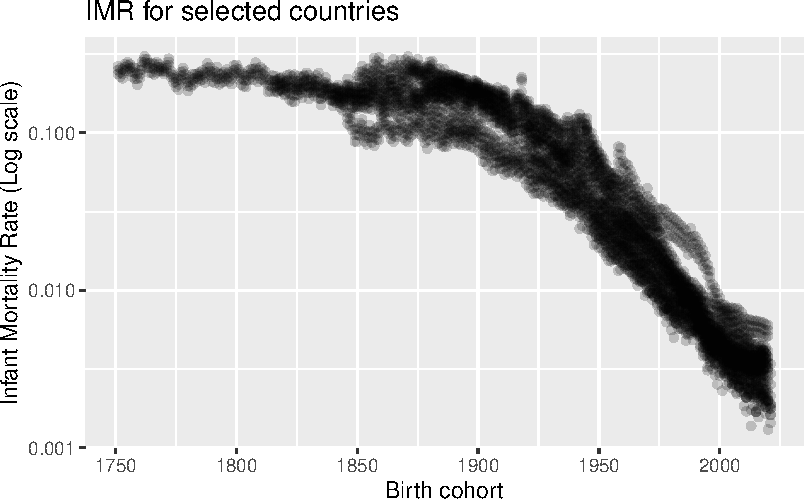
\includegraphics{main_notebook_files/figure-pdf/unnamed-chunk-4-1.pdf}

}

\end{figure}

We should maybe focus on post 1970, and look at sex separately.

\begin{Shaded}
\begin{Highlighting}[]
\NormalTok{lx\_par\_df }\SpecialCharTok{|\textgreater{}} 
  \FunctionTok{mutate}\NormalTok{(}
    \AttributeTok{imr =}\NormalTok{ deaths }\SpecialCharTok{/}\NormalTok{ exposures}
\NormalTok{  ) }\SpecialCharTok{|\textgreater{}} 
  \FunctionTok{filter}\NormalTok{(sex }\SpecialCharTok{!=} \StringTok{\textquotesingle{}total\textquotesingle{}}\NormalTok{) }\SpecialCharTok{|\textgreater{}} 
  \FunctionTok{filter}\NormalTok{(cohort }\SpecialCharTok{\textgreater{}=} \DecValTok{1970}\NormalTok{) }\SpecialCharTok{|\textgreater{}} 
  \FunctionTok{ggplot}\NormalTok{(}\FunctionTok{aes}\NormalTok{(}\AttributeTok{x =}\NormalTok{ cohort, }\AttributeTok{y =}\NormalTok{ imr, }\AttributeTok{group =} \FunctionTok{paste0}\NormalTok{(code, sex), }\AttributeTok{colour =}\NormalTok{ sex)) }\SpecialCharTok{+} 
  \FunctionTok{geom\_line}\NormalTok{() }\SpecialCharTok{+}
  \FunctionTok{scale\_y\_log10}\NormalTok{() }\SpecialCharTok{+} 
  \FunctionTok{facet\_wrap}\NormalTok{(}\SpecialCharTok{\textasciitilde{}}\NormalTok{code) }\SpecialCharTok{+} 
  \FunctionTok{labs}\NormalTok{(}\AttributeTok{x =} \StringTok{"Birth cohort"}\NormalTok{, }\AttributeTok{y =} \StringTok{"Infant Mortality Rate (Log scale)"}\NormalTok{,}
       \AttributeTok{title =} \StringTok{"IMR for selected countries"}\NormalTok{)}
\end{Highlighting}
\end{Shaded}

\begin{figure}[H]

{\centering 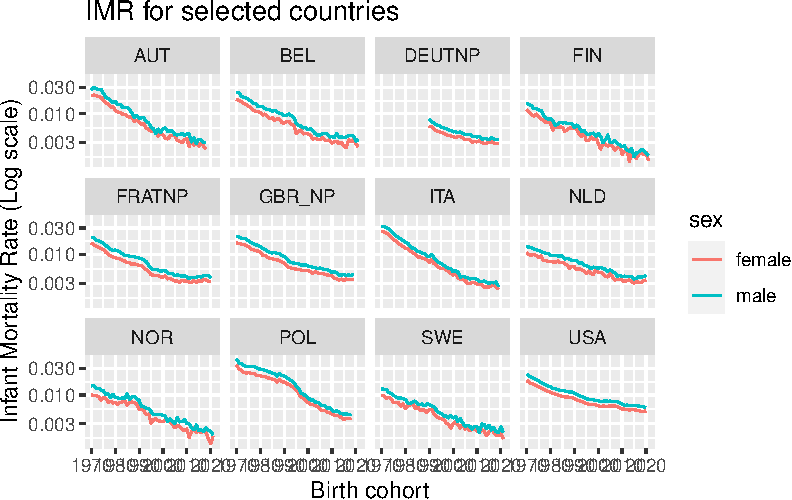
\includegraphics{main_notebook_files/figure-pdf/unnamed-chunk-5-1.pdf}

}

\end{figure}

So, in log space, for each country, male IMRs look like female IMRs, but
shifted up by a given amount.

This given amount looks similar for all countries. This is a simplifying
assumption we can make.

Another simplifying/stylising assumption we can make is that mortality
trends over time is log linear. Country effects then further adjust
upwards or downwards from this general trend. (This are simply
assumptions we can then develop further and critique afterwards. But
they're reasonable starting places.)

We can select a reference country. I think this should be Norway (and
aspirational reference country!).

\hypertarget{modelling-and-model-predictions}{%
\subsection{Modelling and model
predictions}\label{modelling-and-model-predictions}}

\hypertarget{running-linear-regression-models}{%
\subsubsection{Running linear regression
models}\label{running-linear-regression-models}}

We can start with simple linear regression

\begin{Shaded}
\begin{Highlighting}[]
\NormalTok{training\_data }\OtherTok{\textless{}{-}} 
\NormalTok{  lx\_par\_df }\SpecialCharTok{|\textgreater{}} 
  \FunctionTok{mutate}\NormalTok{(}
    \AttributeTok{imr =}\NormalTok{ deaths }\SpecialCharTok{/}\NormalTok{ exposures}
\NormalTok{  ) }\SpecialCharTok{|\textgreater{}} 
  \FunctionTok{filter}\NormalTok{(sex }\SpecialCharTok{!=} \StringTok{\textquotesingle{}total\textquotesingle{}}\NormalTok{) }\SpecialCharTok{|\textgreater{}} 
  \FunctionTok{filter}\NormalTok{(cohort }\SpecialCharTok{\textgreater{}=} \DecValTok{1970}\NormalTok{) }\SpecialCharTok{|\textgreater{}} 
  \FunctionTok{mutate}\NormalTok{(}\AttributeTok{yrs\_since\_1970 =}\NormalTok{ cohort }\SpecialCharTok{{-}} \DecValTok{1970}\NormalTok{) }\SpecialCharTok{|\textgreater{}} 
  \FunctionTok{mutate}\NormalTok{(}\AttributeTok{code =} \FunctionTok{factor}\NormalTok{(code)) }\SpecialCharTok{|\textgreater{}} 
  \FunctionTok{mutate}\NormalTok{(}\AttributeTok{code =} \FunctionTok{relevel}\NormalTok{(code, }\StringTok{"NOR"}\NormalTok{))}

\CommentTok{\# First model: only time matters}
\NormalTok{mod\_00 }\OtherTok{\textless{}{-}} \FunctionTok{lm}\NormalTok{(}\FunctionTok{log}\NormalTok{(imr) }\SpecialCharTok{\textasciitilde{}}\NormalTok{ yrs\_since\_1970, }
             \AttributeTok{data =}\NormalTok{ training\_data)}

\CommentTok{\# Second model: sex also matters }
\NormalTok{mod\_01 }\OtherTok{\textless{}{-}} \FunctionTok{lm}\NormalTok{(}\FunctionTok{log}\NormalTok{(imr) }\SpecialCharTok{\textasciitilde{}}\NormalTok{ yrs\_since\_1970 }\SpecialCharTok{+}\NormalTok{ sex, }
             \AttributeTok{data =}\NormalTok{ training\_data)}

\CommentTok{\# Third model: country also matters}
\NormalTok{mod\_02 }\OtherTok{\textless{}{-}} \FunctionTok{lm}\NormalTok{(}\FunctionTok{log}\NormalTok{(imr) }\SpecialCharTok{\textasciitilde{}}\NormalTok{ yrs\_since\_1970 }\SpecialCharTok{+}\NormalTok{ sex }\SpecialCharTok{+}\NormalTok{ code, }
             \AttributeTok{data =}\NormalTok{ training\_data)}
\end{Highlighting}
\end{Shaded}

\hypertarget{comparing-models}{%
\subsubsection{Comparing models}\label{comparing-models}}

Each of the above models is more complex (parameterised) than the last.
We can test whether the greater complexity is justified using F-tests
(via ANOVA) and using something like BIC and AIC

\begin{Shaded}
\begin{Highlighting}[]
\FunctionTok{anova}\NormalTok{(mod\_00, mod\_01)}
\end{Highlighting}
\end{Shaded}

\begin{verbatim}
Analysis of Variance Table

Model 1: log(imr) ~ yrs_since_1970
Model 2: log(imr) ~ yrs_since_1970 + sex
  Res.Df    RSS Df Sum of Sq      F    Pr(>F)    
1   1176 139.76                                  
2   1175 124.64  1    15.117 142.51 < 2.2e-16 ***
---
Signif. codes:  0 '***' 0.001 '**' 0.01 '*' 0.05 '.' 0.1 ' ' 1
\end{verbatim}

\begin{Shaded}
\begin{Highlighting}[]
\CommentTok{\# Significantly better going from model 00 to model 01}
\FunctionTok{anova}\NormalTok{(mod\_01, mod\_02)}
\end{Highlighting}
\end{Shaded}

\begin{verbatim}
Analysis of Variance Table

Model 1: log(imr) ~ yrs_since_1970 + sex
Model 2: log(imr) ~ yrs_since_1970 + sex + code
  Res.Df     RSS Df Sum of Sq      F    Pr(>F)    
1   1175 124.642                                  
2   1164  34.061 11    90.581 281.41 < 2.2e-16 ***
---
Signif. codes:  0 '***' 0.001 '**' 0.01 '*' 0.05 '.' 0.1 ' ' 1
\end{verbatim}

\begin{Shaded}
\begin{Highlighting}[]
\CommentTok{\# Significantly better going from model 01 to model 02}

\FunctionTok{AIC}\NormalTok{(mod\_00, mod\_01, mod\_02)}
\end{Highlighting}
\end{Shaded}

\begin{verbatim}
       df       AIC
mod_00  3  837.9330
mod_01  4  705.0831
mod_02 15 -801.1207
\end{verbatim}

\begin{Shaded}
\begin{Highlighting}[]
\CommentTok{\# Mod 02 much better than the other two models}
\FunctionTok{BIC}\NormalTok{(mod\_00, mod\_01, mod\_02)}
\end{Highlighting}
\end{Shaded}

\begin{verbatim}
       df       BIC
mod_00  3  853.1477
mod_01  4  725.3694
mod_02 15 -725.0471
\end{verbatim}

\begin{Shaded}
\begin{Highlighting}[]
\CommentTok{\# Mod 02 much better than the other two models}
\end{Highlighting}
\end{Shaded}

The above all indicate country effects should be included.

\hypertarget{interpreting-model-output}{%
\subsubsection{Interpreting model
output}\label{interpreting-model-output}}

The best of the three models has the following summary output

\begin{Shaded}
\begin{Highlighting}[]
\FunctionTok{summary}\NormalTok{(mod\_02)}
\end{Highlighting}
\end{Shaded}

\begin{verbatim}

Call:
lm(formula = log(imr) ~ yrs_since_1970 + sex + code, data = training_data)

Residuals:
     Min       1Q   Median       3Q      Max 
-0.46509 -0.11908 -0.01855  0.10214  0.52216 

Coefficients:
                 Estimate Std. Error  t value Pr(>|t|)    
(Intercept)    -4.5093895  0.0195899 -230.190  < 2e-16 ***
yrs_since_1970 -0.0376992  0.0003454 -109.162  < 2e-16 ***
sexmale         0.2265635  0.0099681   22.729  < 2e-16 ***
codeAUT         0.3460287  0.0240880   14.365  < 2e-16 ***
codeBEL         0.3316310  0.0237221   13.980  < 2e-16 ***
codeDEUTNP      0.2018375  0.0279058    7.233 8.56e-13 ***
codeFIN        -0.1029358  0.0237221   -4.339 1.55e-05 ***
codeFRATNP      0.2476061  0.0238387   10.387  < 2e-16 ***
codeGBR_NP      0.3874066  0.0239606   16.168  < 2e-16 ***
codeITA         0.3610769  0.0239606   15.070  < 2e-16 ***
codeNLD         0.2029796  0.0238387    8.515  < 2e-16 ***
codePOL         0.8997065  0.0240880   37.351  < 2e-16 ***
codeSWE        -0.0955273  0.0237221   -4.027 6.02e-05 ***
codeUSA         0.6143548  0.0238387   25.771  < 2e-16 ***
---
Signif. codes:  0 '***' 0.001 '**' 0.01 '*' 0.05 '.' 0.1 ' ' 1

Residual standard error: 0.1711 on 1164 degrees of freedom
Multiple R-squared:  0.9332,    Adjusted R-squared:  0.9324 
F-statistic:  1250 on 13 and 1164 DF,  p-value: < 2.2e-16
\end{verbatim}

The model predicts that, each year, log IMR falls by -0.0376992. The
exponent of this is 0.9630026, so on average each year IMR falls by
about 3.7\% compared with the previous year.

\textbf{Note: To test for slowdown, include additional time-related
terms, such as whether the year is 2012 or after. Then use ANOVA/AIC/BIC
to see if the additional term is justified by better fit.}

Similarly, the exponents of the sex and country terms indicate what \%
higher or lower male IMR is than female, and how much higher it is in
specific countries compared with Norway.

\begin{Shaded}
\begin{Highlighting}[]
\NormalTok{implied\_hazard\_shifts }\OtherTok{\textless{}{-}} 
\NormalTok{  broom}\SpecialCharTok{::}\FunctionTok{tidy}\NormalTok{(mod\_02) }\SpecialCharTok{|\textgreater{}} 
    \FunctionTok{filter}\NormalTok{(}\FunctionTok{str\_detect}\NormalTok{(term, }\StringTok{"code|sex"}\NormalTok{) ) }\SpecialCharTok{|\textgreater{}} 
    \FunctionTok{mutate}\NormalTok{(}\AttributeTok{term =} \FunctionTok{str\_remove}\NormalTok{(term, }\StringTok{"sex"}\NormalTok{)) }\SpecialCharTok{|\textgreater{}} 
    \FunctionTok{mutate}\NormalTok{(}\AttributeTok{term =} \FunctionTok{str\_remove}\NormalTok{(term, }\StringTok{"code"}\NormalTok{)) }\SpecialCharTok{|\textgreater{}} 
    \FunctionTok{select}\NormalTok{(term, estimate) }\SpecialCharTok{|\textgreater{}} 
    \FunctionTok{mutate}\NormalTok{(}\AttributeTok{hazard\_shift =} \FunctionTok{exp}\NormalTok{(estimate)) }\SpecialCharTok{|\textgreater{}} 
    \FunctionTok{arrange}\NormalTok{(}\FunctionTok{desc}\NormalTok{(hazard\_shift)) }

\NormalTok{implied\_hazard\_shifts}
\end{Highlighting}
\end{Shaded}

\begin{verbatim}
# A tibble: 12 x 3
   term   estimate hazard_shift
   <chr>     <dbl>        <dbl>
 1 POL      0.900         2.46 
 2 USA      0.614         1.85 
 3 GBR_NP   0.387         1.47 
 4 ITA      0.361         1.43 
 5 AUT      0.346         1.41 
 6 BEL      0.332         1.39 
 7 FRATNP   0.248         1.28 
 8 male     0.227         1.25 
 9 NLD      0.203         1.23 
10 DEUTNP   0.202         1.22 
11 SWE     -0.0955        0.909
12 FIN     -0.103         0.902
\end{verbatim}

Over this time period, IMRs in Poland are on average 146\% higher (100 *
(2.46 - 1)) than for the reference country, Norway. The next highest
increased risk is living in the USA, where the IMR risks are 85\% higher
then in Norway, then in the UK (GBR\_NP), where the risks are 47\%
higher. Only Sweden and Finland have lower IMR risks then Norway, with
IMR risks around 9-10\% lower.

For comparison, the male IMR is on average higher 25\% than the
corresponding female IMR.

\hypertarget{examples-of-more-complex-models-e.g.-to-test-austerity-hypotheses}{%
\subsubsection{Examples of more complex models (e.g.~to test Austerity
hypotheses)}\label{examples-of-more-complex-models-e.g.-to-test-austerity-hypotheses}}

We can consider specifications that `flag' years after 2012 as different
from previous years. We can also look at specifications where these
flags apply differently by countries.

\begin{Shaded}
\begin{Highlighting}[]
\NormalTok{mod\_03 }\OtherTok{\textless{}{-}} \FunctionTok{lm}\NormalTok{(}\FunctionTok{log}\NormalTok{(imr) }\SpecialCharTok{\textasciitilde{}}\NormalTok{ yrs\_since\_1970 }\SpecialCharTok{+}\NormalTok{ sex }\SpecialCharTok{+}\NormalTok{ code }\SpecialCharTok{+}\NormalTok{ post\_2012, }
             \CommentTok{\#post\_2012 is our \textquotesingle{}flag\textquotesingle{}}
             \AttributeTok{data =}\NormalTok{ training\_data }\SpecialCharTok{|\textgreater{}} 
               \FunctionTok{mutate}\NormalTok{(}\AttributeTok{post\_2012 =}\NormalTok{ cohort }\SpecialCharTok{\textgreater{}=} \DecValTok{2012}\NormalTok{)}
\NormalTok{          )}

\NormalTok{mod\_04 }\OtherTok{\textless{}{-}} \FunctionTok{lm}\NormalTok{(}\FunctionTok{log}\NormalTok{(imr) }\SpecialCharTok{\textasciitilde{}}\NormalTok{ yrs\_since\_1970 }\SpecialCharTok{+}\NormalTok{ sex }\SpecialCharTok{+}\NormalTok{ code }\SpecialCharTok{*}\NormalTok{ post\_2012, }
             \CommentTok{\#post\_2012 is our \textquotesingle{}flag\textquotesingle{}. The * after code means it interacts with country (i.e. is experienced differently in) different countries}
             \AttributeTok{data =}\NormalTok{ training\_data }\SpecialCharTok{|\textgreater{}} 
               \FunctionTok{mutate}\NormalTok{(}\AttributeTok{post\_2012 =}\NormalTok{ cohort }\SpecialCharTok{\textgreater{}=} \DecValTok{2012}\NormalTok{)}
             \CommentTok{\# n.b. we can just about use cohort as year as looking at IMR}
\NormalTok{          )}
\end{Highlighting}
\end{Shaded}

We can compare these models using the same strategy as before:

\begin{Shaded}
\begin{Highlighting}[]
\FunctionTok{anova}\NormalTok{(mod\_02, mod\_03)}
\end{Highlighting}
\end{Shaded}

\begin{verbatim}
Analysis of Variance Table

Model 1: log(imr) ~ yrs_since_1970 + sex + code
Model 2: log(imr) ~ yrs_since_1970 + sex + code + post_2012
  Res.Df    RSS Df Sum of Sq      F    Pr(>F)    
1   1164 34.061                                  
2   1163 29.523  1    4.5384 178.78 < 2.2e-16 ***
---
Signif. codes:  0 '***' 0.001 '**' 0.01 '*' 0.05 '.' 0.1 ' ' 1
\end{verbatim}

\begin{Shaded}
\begin{Highlighting}[]
\CommentTok{\# significantly better}
\FunctionTok{anova}\NormalTok{(mod\_03, mod\_04)}
\end{Highlighting}
\end{Shaded}

\begin{verbatim}
Analysis of Variance Table

Model 1: log(imr) ~ yrs_since_1970 + sex + code + post_2012
Model 2: log(imr) ~ yrs_since_1970 + sex + code * post_2012
  Res.Df    RSS Df Sum of Sq      F    Pr(>F)    
1   1163 29.523                                  
2   1152 22.415 11    7.1083 33.212 < 2.2e-16 ***
---
Signif. codes:  0 '***' 0.001 '**' 0.01 '*' 0.05 '.' 0.1 ' ' 1
\end{verbatim}

\begin{Shaded}
\begin{Highlighting}[]
\CommentTok{\# also significnatly better }

\FunctionTok{AIC}\NormalTok{(mod\_00, mod\_01, mod\_02, mod\_03, mod\_04)}
\end{Highlighting}
\end{Shaded}

\begin{verbatim}
       df        AIC
mod_00  3   837.9330
mod_01  4   705.0831
mod_02 15  -801.1207
mod_03 16  -967.5715
mod_04 27 -1270.0583
\end{verbatim}

\begin{Shaded}
\begin{Highlighting}[]
\FunctionTok{BIC}\NormalTok{(mod\_00, mod\_01, mod\_02, mod\_03, mod\_04)}
\end{Highlighting}
\end{Shaded}

\begin{verbatim}
       df        BIC
mod_00  3   853.1477
mod_01  4   725.3694
mod_02 15  -725.0471
mod_03 16  -886.4263
mod_04 27 -1133.1258
\end{verbatim}

\begin{Shaded}
\begin{Highlighting}[]
\CommentTok{\# The most complex also preferred}
\end{Highlighting}
\end{Shaded}

\begin{Shaded}
\begin{Highlighting}[]
\FunctionTok{summary}\NormalTok{(mod\_04)}
\end{Highlighting}
\end{Shaded}

\begin{verbatim}

Call:
lm(formula = log(imr) ~ yrs_since_1970 + sex + code * post_2012, 
    data = mutate(training_data, post_2012 = cohort >= 2012))

Residuals:
     Min       1Q   Median       3Q      Max 
-0.45053 -0.08771 -0.00708  0.08331  0.43355 

Coefficients:
                           Estimate Std. Error  t value Pr(>|t|)    
(Intercept)              -4.4366654  0.0175218 -253.208  < 2e-16 ***
yrs_since_1970           -0.0414092  0.0003743 -110.642  < 2e-16 ***
sexmale                   0.2265635  0.0081282   27.874  < 2e-16 ***
codeAUT                   0.3589119  0.0215235   16.675  < 2e-16 ***
codeBEL                   0.3070072  0.0215235   14.264  < 2e-16 ***
codeDEUTNP                0.1783128  0.0262268    6.799 1.69e-11 ***
codeFIN                  -0.0990956  0.0215235   -4.604 4.60e-06 ***
codeFRATNP                0.1953260  0.0215235    9.075  < 2e-16 ***
codeGBR_NP                0.3576237  0.0215235   16.615  < 2e-16 ***
codeITA                   0.3864829  0.0215235   17.956  < 2e-16 ***
codeNLD                   0.1444401  0.0215235    6.711 3.03e-11 ***
codePOL                   0.9476619  0.0215235   44.029  < 2e-16 ***
codeSWE                  -0.1280075  0.0215235   -5.947 3.61e-09 ***
codeUSA                   0.5409430  0.0215235   25.133  < 2e-16 ***
post_2012TRUE             0.1137773  0.0360440    3.157 0.001638 ** 
codeAUT:post_2012TRUE    -0.0897526  0.0531622   -1.688 0.091628 .  
codeBEL:post_2012TRUE     0.1280435  0.0490812    2.609 0.009203 ** 
codeDEUTNP:post_2012TRUE  0.1817031  0.0536628    3.386 0.000733 ***
codeFIN:post_2012TRUE    -0.0199693  0.0490812   -0.407 0.684184    
codeFRATNP:post_2012TRUE  0.2959535  0.0501707    5.899 4.80e-09 ***
codeGBR_NP:post_2012TRUE  0.1859303  0.0515007    3.610 0.000319 ***
codeITA:post_2012TRUE    -0.1590001  0.0515007   -3.087 0.002068 ** 
codeNLD:post_2012TRUE     0.3314227  0.0501707    6.606 6.02e-11 ***
codePOL:post_2012TRUE    -0.3352580  0.0531622   -6.306 4.06e-10 ***
codeSWE:post_2012TRUE     0.1688973  0.0490812    3.441 0.000600 ***
codeUSA:post_2012TRUE     0.4156994  0.0501707    8.286 3.23e-16 ***
---
Signif. codes:  0 '***' 0.001 '**' 0.01 '*' 0.05 '.' 0.1 ' ' 1

Residual standard error: 0.1395 on 1152 degrees of freedom
Multiple R-squared:  0.956, Adjusted R-squared:  0.9551 
F-statistic:  1001 on 25 and 1152 DF,  p-value: < 2.2e-16
\end{verbatim}

Because of the presence of interaction terms, the coefficients are now
somewhat harder to interpret directly. Instead, we can look at the
predicted values they imply, and how they differ between countries.

\hypertarget{showing-what-a-model-specification-predicts}{%
\subsubsection{Showing what a model specification
predicts}\label{showing-what-a-model-specification-predicts}}

\begin{Shaded}
\begin{Highlighting}[]
\NormalTok{pred\_df }\OtherTok{\textless{}{-}} 
  \FunctionTok{expand\_grid}\NormalTok{(}
    \AttributeTok{cohort =} \DecValTok{1990}\SpecialCharTok{:}\DecValTok{2022}\NormalTok{, }
    \AttributeTok{sex =} \FunctionTok{c}\NormalTok{(}\StringTok{"male"}\NormalTok{, }\StringTok{"female"}\NormalTok{),}
    \AttributeTok{code =} \FunctionTok{c}\NormalTok{(}
    \StringTok{"AUT"}\NormalTok{, }\CommentTok{\#Austria}
    \StringTok{"BEL"}\NormalTok{, }\CommentTok{\#Belgium}
    \StringTok{"FIN"}\NormalTok{, }\CommentTok{\#Finland}
    \StringTok{"FRATNP"}\NormalTok{, }\CommentTok{\#France}
    \StringTok{"DEUTNP"}\NormalTok{, }\CommentTok{\#Germany}
    \StringTok{"ITA"}\NormalTok{, }\CommentTok{\#Italy}
    \StringTok{"NLD"}\NormalTok{, }\CommentTok{\#Netherlands}
    \StringTok{"NOR"}\NormalTok{, }\CommentTok{\#Norway}
    \StringTok{"POL"}\NormalTok{, }\CommentTok{\#Poland}
    \StringTok{"SWE"}\NormalTok{, }\CommentTok{\#Sweden}
    \StringTok{"USA"}\NormalTok{, }\CommentTok{\#USA}
    \StringTok{"GBR\_NP"} \CommentTok{\#UK}
\NormalTok{    )}
\NormalTok{  )  }\SpecialCharTok{|\textgreater{}} 
  \FunctionTok{mutate}\NormalTok{(}
    \AttributeTok{yrs\_since\_1970 =}\NormalTok{ cohort }\SpecialCharTok{{-}} \DecValTok{1970}\NormalTok{,}
    \AttributeTok{post\_2012 =}\NormalTok{ cohort }\SpecialCharTok{\textgreater{}=} \DecValTok{2012}
\NormalTok{  )}

\NormalTok{preds }\OtherTok{\textless{}{-}} \FunctionTok{predict}\NormalTok{(mod\_04, }\AttributeTok{newdata =}\NormalTok{ pred\_df)}

\NormalTok{preds\_pred\_df }\OtherTok{\textless{}{-}} 
\NormalTok{  pred\_df }\SpecialCharTok{|\textgreater{}} 
  \FunctionTok{mutate}\NormalTok{(}
    \AttributeTok{pred\_limr =}\NormalTok{ preds}
\NormalTok{  )}
\end{Highlighting}
\end{Shaded}

Now to visualise

\begin{Shaded}
\begin{Highlighting}[]
\NormalTok{preds\_pred\_df }\SpecialCharTok{|\textgreater{}} 
  \FunctionTok{left\_join}\NormalTok{(training\_data) }\SpecialCharTok{|\textgreater{}} 
  \FunctionTok{mutate}\NormalTok{(}
    \AttributeTok{obs\_limr =} \FunctionTok{log}\NormalTok{(imr)}
\NormalTok{  ) }\SpecialCharTok{|\textgreater{}} 
  \FunctionTok{ggplot}\NormalTok{(}\FunctionTok{aes}\NormalTok{(}\AttributeTok{x =}\NormalTok{ cohort, }\AttributeTok{color =}\NormalTok{ sex)) }\SpecialCharTok{+} 
  \FunctionTok{geom\_point}\NormalTok{(}\FunctionTok{aes}\NormalTok{(}\AttributeTok{y =}\NormalTok{ obs\_limr)) }\SpecialCharTok{+} 
  \FunctionTok{geom\_line}\NormalTok{(}\FunctionTok{aes}\NormalTok{(}\AttributeTok{y =}\NormalTok{ pred\_limr)) }\SpecialCharTok{+} 
  \FunctionTok{facet\_wrap}\NormalTok{(}\SpecialCharTok{\textasciitilde{}}\NormalTok{code) }\SpecialCharTok{+} 
  \FunctionTok{labs}\NormalTok{(}\AttributeTok{x =} \StringTok{"Birth cohort"}\NormalTok{, }
       \AttributeTok{y =} \StringTok{"Log IMR"}\NormalTok{,}
       \AttributeTok{title =} \StringTok{"Observed and predicted Log IMR for selected countries"}\NormalTok{,}
       \AttributeTok{subtitle =} \StringTok{"Points: Observed. Lines: Predicted"}\NormalTok{)}
\end{Highlighting}
\end{Shaded}

\begin{verbatim}
Joining with `by = join_by(cohort, sex, code, yrs_since_1970)`
\end{verbatim}

\begin{verbatim}
Warning: Removed 54 rows containing missing values (`geom_point()`).
\end{verbatim}

\begin{figure}[H]

{\centering 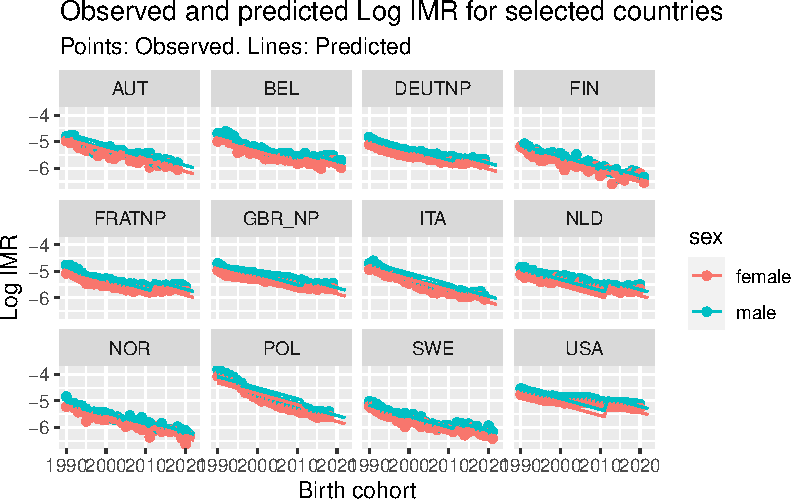
\includegraphics{main_notebook_files/figure-pdf/unnamed-chunk-14-1.pdf}

}

\end{figure}

The lines showing the model predictions show the importance of
structural assumptions in the model. The model assumes a constant annual
rate of mortality improvement throughout the whole series, and then
allows the line over time to be moved upwards or downwards in log space
for 2012 onwards.

\hypertarget{deciding-whether-a-more-complex-model-is-worth-its-additional-complexity}{%
\subsubsection{Deciding whether a more complex model is worth its
additional
complexity}\label{deciding-whether-a-more-complex-model-is-worth-its-additional-complexity}}

For countries where there has been slowdown after around 2012, this
structural assumption might not be appropriate. Instead we should
consider models in which the rate of improvement over time itself is
allowed to be different after 2012 than before. As before we can build
this model specification and compared the penalised fit.

\begin{Shaded}
\begin{Highlighting}[]
\NormalTok{mod\_05 }\OtherTok{\textless{}{-}}  \FunctionTok{lm}\NormalTok{(}\FunctionTok{log}\NormalTok{(imr) }\SpecialCharTok{\textasciitilde{}}\NormalTok{ yrs\_since\_1970 }\SpecialCharTok{+}\NormalTok{ sex }\SpecialCharTok{+}\NormalTok{ code }\SpecialCharTok{*}\NormalTok{ yrs\_since\_2012, }
              \CommentTok{\#Now using yrs\_since\_2012, which allows change in slope not just intercept}
             \AttributeTok{data =}\NormalTok{ training\_data }\SpecialCharTok{|\textgreater{}} 
               \FunctionTok{mutate}\NormalTok{(}
                 \AttributeTok{post\_2012 =}\NormalTok{ cohort }\SpecialCharTok{\textgreater{}=} \DecValTok{2012}\NormalTok{,}
                 \AttributeTok{yrs\_since\_2012 =} \FunctionTok{ifelse}\NormalTok{(}
\NormalTok{                   post\_2012, }
\NormalTok{                   cohort }\SpecialCharTok{{-}} \DecValTok{2012}\NormalTok{,}
                   \DecValTok{0}
\NormalTok{                  )}
\NormalTok{                 )}
             \CommentTok{\# n.b. we can just about use cohort as year as looking at IMR}
\NormalTok{          )}
\end{Highlighting}
\end{Shaded}

Compare the models

\begin{Shaded}
\begin{Highlighting}[]
\FunctionTok{AIC}\NormalTok{(}
\NormalTok{  mod\_00, mod\_01, mod\_02, mod\_03, mod\_04, mod\_05}
\NormalTok{)}
\end{Highlighting}
\end{Shaded}

\begin{verbatim}
       df        AIC
mod_00  3   837.9330
mod_01  4   705.0831
mod_02 15  -801.1207
mod_03 16  -967.5715
mod_04 27 -1270.0583
mod_05 27 -1210.8527
\end{verbatim}

\begin{Shaded}
\begin{Highlighting}[]
\FunctionTok{BIC}\NormalTok{(}
\NormalTok{  mod\_00, mod\_01, mod\_02, mod\_03, mod\_04, mod\_05}
\NormalTok{)}
\end{Highlighting}
\end{Shaded}

\begin{verbatim}
       df        BIC
mod_00  3   853.1477
mod_01  4   725.3694
mod_02 15  -725.0471
mod_03 16  -886.4263
mod_04 27 -1133.1258
mod_05 27 -1073.9203
\end{verbatim}

The model allowing a different slope for post 2012 doesn't outperform
the simpler model which simply adjusts the trend upwards or downwards.
This suggests that the simpler model may be `good enough' for producing
summary estimates of how large any post 2012 slowdown may have been in
IMR trends for different countries, even though it's qualitatively not
quite the pattern we see in the data.

Further model specifications, representing different theories about
these trends and how they differ between places, can also be tried. In
particular models including one or more breakpoints in the IMR trends
may be worth looking at, as in
\href{https://www.dannydorling.org/wp-content/files/dannydorling_publication_id9575.pdf}{this
paper}. (i.e.~the code in that paper, which looks at \(e_0\) and
\(e_{65}\), could also be applied to IMR trends as well.)

\hypertarget{summarising-the-good-enough-model}{%
\subsubsection{Summarising the `good enough'
model}\label{summarising-the-good-enough-model}}

Model 04, which is structurally overly `stylised' (i.e.~doesn't look
right) but still preferred over the more complex model 05, allows for
single summary estimates of what's happened to IMR trends post 2012. Or
more specifically by what \% earlier trends were `set back' compared
with the pre 2012 period.

As Norway is the reference category, we know the coefficient
\texttt{post\_2012TRUE} corresponds to Norway. This coefficient is about
0.0114. The exponent of this is 1.12, so around a 12\% higher IMR for
Norway compared with the pre 2012 trend.

For other countries, the \texttt{post\_2012TRUE} coefficient needs to be
added to the country-specific coefficient
(e.g.~\texttt{post\_2012TRUE\ +\ codeGBR\_NP:post\_2012TRUE} for the
UK), before exponentiating.

For the UK the estimate of how much IMRs were set back from 2012 onwards
is \texttt{exp(0.1137773\ +\ 0.1859303)} , which is 1.349, suggesting
that from 2012 IMRs were around 35\% higher than the long-term trend.

The following code shows the same for all other countries

\begin{Shaded}
\begin{Highlighting}[]
\NormalTok{broom}\SpecialCharTok{::}\FunctionTok{tidy}\NormalTok{(mod\_04) }\SpecialCharTok{|\textgreater{}} 
  \FunctionTok{filter}\NormalTok{(}\FunctionTok{str\_detect}\NormalTok{(term, }\StringTok{"post\_2012"}\NormalTok{)) }\SpecialCharTok{|\textgreater{}} 
  \FunctionTok{mutate}\NormalTok{(}
    \AttributeTok{code =} \FunctionTok{str\_remove}\NormalTok{(term, }\StringTok{"post\_2012TRUE"}\NormalTok{),}
    \AttributeTok{code =} \FunctionTok{str\_remove}\NormalTok{(code, }\StringTok{"code"}\NormalTok{),}
    \AttributeTok{code =} \FunctionTok{str\_remove}\NormalTok{(code, }\StringTok{":"}\NormalTok{),}
    \AttributeTok{code =} \FunctionTok{ifelse}\NormalTok{(code }\SpecialCharTok{==} \StringTok{""}\NormalTok{, }\StringTok{"NOR"}\NormalTok{, code)}
\NormalTok{  ) }\SpecialCharTok{|\textgreater{}} 
  \FunctionTok{mutate}\NormalTok{(}
    \AttributeTok{delta =} \FunctionTok{ifelse}\NormalTok{(}
\NormalTok{      code }\SpecialCharTok{==} \StringTok{"NOR"}\NormalTok{, }
\NormalTok{      estimate,}
\NormalTok{      estimate }\SpecialCharTok{+}\NormalTok{ estimate[code }\SpecialCharTok{==} \StringTok{"NOR"}\NormalTok{]}
\NormalTok{    )}
\NormalTok{  ) }\SpecialCharTok{|\textgreater{}} 
  \FunctionTok{mutate}\NormalTok{(}
    \AttributeTok{pct\_change =} \FunctionTok{exp}\NormalTok{(delta) }
\NormalTok{  ) }\SpecialCharTok{|\textgreater{}} 
  \FunctionTok{select}\NormalTok{(code, pct\_change) }\SpecialCharTok{|\textgreater{}} 
  \FunctionTok{arrange}\NormalTok{(}\FunctionTok{desc}\NormalTok{(pct\_change))}
\end{Highlighting}
\end{Shaded}

\begin{verbatim}
# A tibble: 12 x 2
   code   pct_change
   <chr>       <dbl>
 1 USA         1.70 
 2 NLD         1.56 
 3 FRATNP      1.51 
 4 GBR_NP      1.35 
 5 DEUTNP      1.34 
 6 SWE         1.33 
 7 BEL         1.27 
 8 NOR         1.12 
 9 FIN         1.10 
10 AUT         1.02 
11 ITA         0.956
12 POL         0.801
\end{verbatim}

This suggests that the post 2012 period is associated with substantial
setbacks in IMR in almost all countries included, with the exception of
Italy and Poland. The USA has the highest rate of `setback' relative to
earlier trends, with IMR estimated to be around 70\% higher than if
there had not been a setback from 2012.

\hypertarget{summary}{%
\subsection{Summary}\label{summary}}

This notebook includes scripts for:

\begin{itemize}
\item
  Getting data from a standard resource
\item
  Running a series of stylised models of IMR against time
\item
  Producing single parameter summaries of sex and country-specific
  differences in overall trends
\item
  Comparing between different model specifications and trying to find
  the right balance between model complexity and model accuracy
\item
  Producing model predictions and plotting these against observed
  values.
\end{itemize}

The model specifications considered are not the only models worth
considering, and the `best' model presented, model 4, stylises the post
2012 effect in ways that are not especially realistic. However it does
allow single summary estimates of differences both prior and post 2012
between countries, and the general strategy can be adapted to other
countries and datasets.

\hypertarget{not-covered}{%
\subsubsection{Not covered}\label{not-covered}}

\begin{itemize}
\item
  Other ways of comparing model fit (e.g.~RMSE)
\item
  Negative binomial modelling (largely the same specification, but may
  produce more plausible confidence intervals
\end{itemize}

\hypertarget{appendix-downloading-directly-from-hmd}{%
\subsection{Appendix: Downloading directly from
HMD}\label{appendix-downloading-directly-from-hmd}}

The first script downloads directly from the Human Mortality Database.

This requires both registering with the HMD, adding username and
password as environment variables to R, and also a lot of luck. To try
this out do the following:

\begin{enumerate}
\def\labelenumi{\arabic{enumi}.}
\tightlist
\item
  Register with the Human Mortality Database at https://mortality.org.
  Make sure to record username and password
\item
  Within R, and within the console, set the environment variables as
  follows:
\end{enumerate}

\begin{verbatim}
Sys.setenv(HMD_USERNAME = "<WHATEVER YOUR USERNAME IS>")
Sys.setenv(HMD_PASSWORD = "<WHATEVER YOUR PASSWORD IS>")
\end{verbatim}

To test that the environment variables have been set correctly

\begin{verbatim}
Sys.getenv("HMD_USERNAME") # Should return username
Sys.getenv("HMD_PASSWORD") # Should return password
\end{verbatim}

If these are set correctly, then the first chunk of code \emph{should}
work

\begin{enumerate}
\def\labelenumi{\arabic{enumi}.}
\setcounter{enumi}{2}
\tightlist
\item
  To try this in practice, make sure to change \texttt{eval=false} to
  \texttt{eval=true} in this first chunk
\end{enumerate}



\end{document}
